The goal was to estimate muscles activation during one gait cycle from the first heel strike to the end of the swing phase using a 3D one-leg model with 12 DoFs and 17 muscles. 
Pure residual joint torques were also added in addition to muscle-induced ones, to compensate for model weaknesses.
Based on experimental force plateform data and markers position, the stance was divided into three phases (heel, flatfoot and forefoot contacts) of fixed duration (\hl{XXX, XXX and XXX}), to follow the natural rolling movement of the foot from heel strike to toe off.
The interaction between the ground and the foot was modeled using 4 contact points located at the heel and the forefoot (first, fifth metatarsi and hallux).\\ 
The optimization problem consisted in minimizing the errors between predicted $m_p$ and measured $m_m$ markers trajectories, predicted $f_p$, $\tau^f_p$ and measured $f_m$, $\tau^f_m$, respectively ground reaction forces and moments at all contact points.
A regularization term on muscle activations ($a$) was also added (least-activations).
Each phase was discretized into 94 intervals and the objective function was written as follows:

\[ 
\resizebox{0.9\columnwidth}{!}{$ 
\begin{aligned}
\mathcal{J} = &\int_{t=0}^{T}\underbrace{\omega_1(\|m_p - m_m\|^{2})}_{\mathtt{TRACK\_MARKERS}}~ 
+ ~ \underbrace{\omega_2(\|f_p - f_c\|^{2})}_{\mathtt{TRACK\_FORCES}}\\
&+ ~ \underbrace{\omega_3(\|tau^f_p - tau^f_m\|^{2})}_{\mathtt{TRACK\_MOMENTS}}~
+ ~ \underbrace{\omega_4\|a\|^2}_{\mathtt{MIN\_ACTIVATION}}~dt, 
\end{aligned}  
$}  
\addtag  
\label{eq:ocp_walk}  
\]  

where $\omega_1$, $\omega_2$, $\omega_3$, $\omega_4$ are weighting factors and $T$ is the motion duration.
Non-slipping ($\mathtt{NON\_SLIPPING}$) and unilateral contact force ($\mathtt{CONTACT\_FORCE}$) constraints prevented the foot from slipping and penetrating into the ground. 
In between phases, the use of the $\mathtt{IMPACT}$ state transition allowed to represent the gain or loss of contact(s) in the dynamics (e.g., swing phase to heel strike [thesis Felis - articles?]).\\

\hl{commenter les resultats}

(Fig.~\ref{fig:snapshots_multiphase_walking_cycle}). 

\begin{figure*}[t!]
\centering
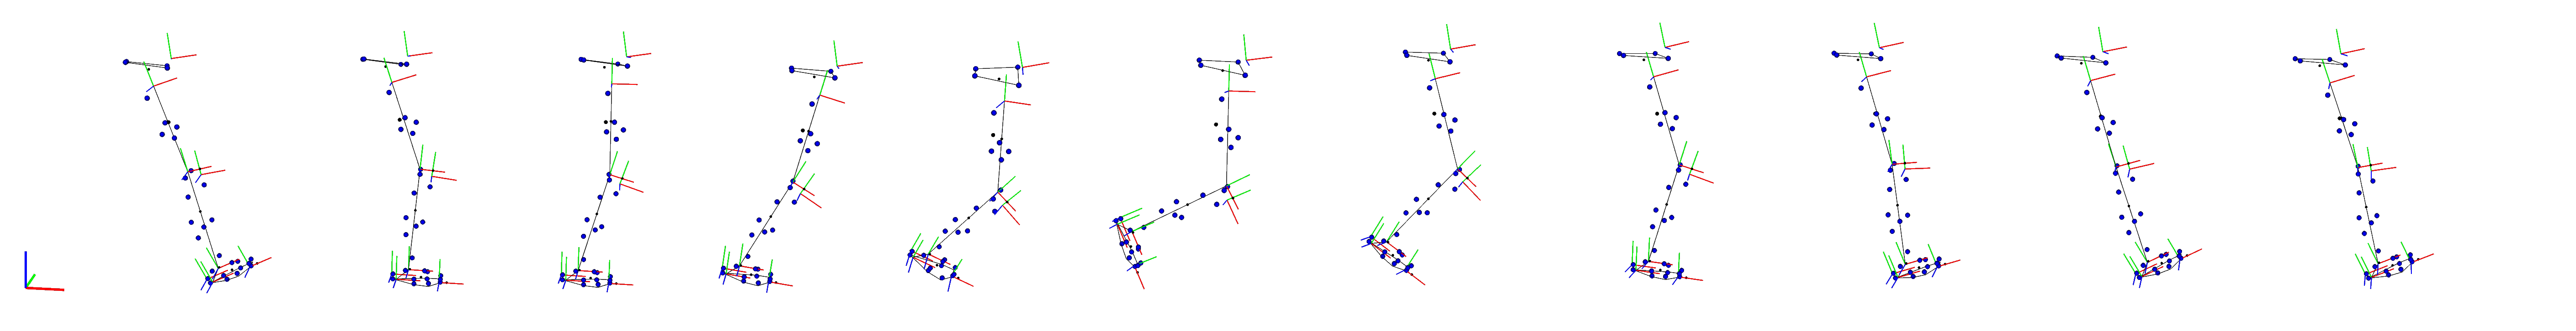
\includegraphics[width=\textwidth]{figures/multiphase_walking_cycle.png}\\
\caption{Snapshots of a walking gait cycle driven by torque actuators.}
\label{fig:snapshots_multiphase_walking_cycle}
\end{figure*}

%\begin{table}[h!]
%\caption{\small Objective terms of the Multiphase torque driven walking cycle }
%\label{tab:Multiphase_torque_driven_walking_cycle}
%\centering
%\begin{tabular}{c c c c}
%\toprule 
%& Type & Function & Weight \\ 
%\midrule
%$\#1$ & Lagrange & TRACK\_ STATE & $1e5$ \\ 
%\midrule
%$\#2$ & Lagrange & MINIMIZE\_ TORQUE\_ DERIVATIVE & $1e-2$ \\ 
%\midrule
%$\#3$ & Lagrange & TRACK\_ GRF & $1e-2$ \\ 
%\midrule
%$\#4$ & Lagrange & TRACK\_ MOMENTS & $1e-1$ \\
%\bottomrule
%\end{tabular}
%\end{table}
